\documentclass[10pt]{report}
\usepackage{graphicx}
\usepackage{a4}
\usepackage{url}
\usepackage{fullpage}

% Report template authored V. Sorge, adapted S. Vickers.

\title{% This is the title of your document
{\normalsize Software Workshop Team Java (06-08165) 2010/11, Dr. E. Thompson}\\[2cm]
Project Report:\\
Space Runner Game}
\author{Team B3:\\
Daniel Cecil\\
Jere Ketonen\\
David Saunders\\
Michal Staniaszek
}

\begin{document}
\maketitle
\chapter*{Work Breakdown}
\label{work-breakdown}

\thispagestyle{empty}

% Obviously these need discussing and changing....
{\small

\noindent\begin{tabular}{|l||l|l|l|l|l|}\hline
  \textbf{Coding} & \textbf{Daniel} & \textbf{Jere} & \textbf{David}
 & \textbf{Michal} \\\hline\hline
 Datastructures & Contribution: 100\% & 0\% & 0\% & 0\%\\\hline
 \ldots & \ldots & \ldots & \ldots & \ldots \\\hline
\end{tabular}\vspace*{1cm}

\noindent\begin{tabular}{|l||l|l|l|l|l|}\hline
  \textbf{Report} & \textbf{Daniel} & \textbf{Jere} & \textbf{David}
 & \textbf{Michal}\\\hline\hline
 Introduction & Chapter~\ref{cha:introduction}: 100\% & 0\% & 0\% & 0\%\\\hline
 \ldots & \ldots & \ldots & \ldots & \ldots \\\hline
\end{tabular}

}     % This is the "}" that matches the "{" before "\small"

\tableofcontents
\thispagestyle{empty}

\begin{abstract}
  You should write a one-page abstract written as an ``Executive Summary''. It
  should be written for someone who is familiar with the Team Java module, so
  that there is no need for background or generalities. Rather, you should
  explain what is special about your project, and what you claim to have
  achieved. (One page maximum.)
\end{abstract}


\chapter{Introduction}
\label{cha:introduction}

This aim of this report is to give a overview of the team Java work we did for 11 weeks on a Space Shooter game and how it progressed from an idea on paper to a functional program.
It will be broken into sections covering important details on the design process, the way we worked and put the project together, the problems we faced, how we over came those problems and how we could improve the project futher with more time and resources.


Give a brief overview and guide the reader to the important points
in the remaining sections.

This template for your report also contains some examples of how to use some
{\LaTeX} elements and commands. In particular, there are examples for tables,
how to include figures, and various environments for bullet points or
enumerations.

For further information (and here is how to do a bullet list):
\begin{itemize}
\item look on the Team Java web page,\\
\url{http://www.cs.bham.ac.uk/internal/courses/team-java/current}\\
  (Click on ``Guidance''.)
\item google ``latex''
\item look at the \LaTeX book \cite{latex}
\end{itemize}


This is how to do numbered lists:
\begin{enumerate}
\item First point
\item Second point
\item \ldots
\end{enumerate}

This is how to do sections:

\section{Some topic}\label{some}

\section{Another topic}\label{another}

If you set a label with the \texttt{label} command, you can then use
the \texttt{ref} command to refer to that section -- e.g.
section~\ref{some}. This means you don't need to know about section
numbers. Note that \texttt{\~} means a space that cannot be broken
across lines.
 % needs doing...
\chapter{Requirements}
\label{cha:requirements}
\section{Functional User Requirements}
\label{sec: functional}

This section outlines the functional requirements which the system will be tested against. Functional requirements are what the system is expected to do and how to user interacts with the software. Each requirement is split into sub-requirements for ease of understanding and clarity.

\begin{enumerate}
\item \textbf{The human player is able to control one's spaceship}
\\* This is a core requirement needed to be able to play the game successfully in at least a single player mode without any crashes or bugs.
\begin{enumerate}
\item The user is able to use either a mouse or the keyboard's arrow keys to move the spaceship.
\item The user's spaceship is able to move freely along the x and y coordinates but not leave the frame's boundaries.
\item The user will be able to hold more than one key for diagonal movement where the movement speed much be normalised.
\item The user's spaceship will be able to be represented graphically on the screen.
\end{enumerate}

\item \textbf{The human player will be able to shoot}
\\* The aim of the game is to enable the user to destroy enemy ships and therefore shooting is a must-have requirement of the game.
\begin{enumerate}
\item The user will be able to shoot by tapping or holding the spacebar or the mouse button (left click).
\item The user's spaceship will have a type of weapon to use, this can be changed during the game (if implemented - dependant on future requirement).
\item The user's shot will follow a set path forwards (negative y-coordinate movement).
\item Shots which leave the frame's boundary will be removed from the game state.
\end{enumerate}

\item \textbf{Enemies will be created to be destroyed by the user}
\\* This is a core functional requirement that needs to be implemented to enable the user to progress through the game by shooting down opposing units.
\begin{enumerate}
\item Enemies will be spawned at set locations on the screen.
\item Enemy units are to have a set health limit.
\item Enemies will be able to be shot by any user spaceship.
\item Enemies are to be distinguishable from friendly user spaceships by using different shapes or graphics.
\item The enemy unit's health will be decreased when a user's shot collides with the enemy.
\item Enemy's will 'die' once all their health have been depleted.
\end{enumerate}

\item \textbf{Enemies are to be able to return a level of resistance}
\\* This requirement is needed to make the game more interesting by introducing the possibility of a player 'death'
\begin{enumerate}
\item Enemies are able to return shots towards the human players with the use of different weapons.
\item Enemies are able to move in certain paths (zig-zag, diagonal, straight, side-to-side).
\item If the player collides with an enemy the player will 'die'
\item 'Boss' enemies are to be introduced which fire more shots and have more health.
\end{enumerate}

\item \textbf{The game is to run continuously with set events occurring at regular intervals}
\\* This requirement ensures the game runs smoothly and that something will always happen. For example, to stop the incidence of no more enemies being spawned (so the game is playable).
\begin{enumerate}
\item The game is to implement a Timer class.
\item Enemies will always be spawned at set intervals during the game. These can be changed to be more or less frequent (if future requirement is implemented).
\item Each tick of the timer will move enemies, player units (depending on user input) and projectiles.
\item The game panel will be redrawn at every tick of the timer.
\end{enumerate}

\item \textbf{The game will be able to be multiplayer across the network}
\\* This requirement is necessary to fulfil the assessment criteria allowing for a second human user to play in co-operative mode with each other against the computer enemies.
\begin{enumerate}
\item Each human user will be able to select whether they will act as the host or the client PC.
\item Clients will be able to enter the Host's IP address to connect.
\item The host's game will start immediately after selection with clients dropping into the game at a set spawn point.
\item The game must be able to support at least two human players and a maximum of eight players (7 clients).
\item All users must be connected to the same LAN network.
\item All users must have similar game information on their screens (player, enemy and projectile positions).
\item With each tick of the timer (requirement 5) each player's screen will be updated with network data from the host.
\end{enumerate}

\item \textbf{The game must have a terminating clause}
\\* This requirement ensures that the game will end at some point.
\begin{enumerate}
\item Once a player's health has been depleted, that unit will 'die' and be removed from the game allowing other player's to carry on playing.
\item If a player collides with an enemy unit they will also 'die'
\item The player's score will be displayed on termination and if high enough will be recorded in a high scores table.
\end{enumerate}

\item \textbf{The game will include a Graphical User Interface (GUI)}
\\* This allows all users to be able to start the necessary game type as well as actually play the game with the information displayed on the screen.
\begin{enumerate}
\item The game will run from a single frame.
\item Panel's are to be added to the frame: Menu, Game, Gameover.
\item The Menu Panel is to feature buttons corresponding to various game types and options.
\item The Menu Panel is to be accessible from within the game (Esc key).
\item The Game is to be able to be paused using the 'P' key.
\item The window is to be resizable allowing for full-screen play.
\item The Game Panel is to feature a scrolling 'star-like' background (black with white stars).
\item The game objects (players, enemies and projectiles) are to be represented by shapes or sprites (graphics).
\end{enumerate}

\end{enumerate}


\subsection{Attributes}
\label{sec: req_attributes}

\noindent\begin{tabular}{| l || p{6cm} | p{7cm} |}\hline
  \textbf{Attribute} & \textbf{Requirement No.} & \textbf{Comment}  \\\hline\hline
  Status & All & Approved - development started \\\hline
 Priority & 1, 2, 3, 4abc, 5, 6, 7, 8abch  - Mandatory. &  Mandatory requirements must be implemented.\\
 & 4d, 8defg - Important & \\\hline
 Effort & All & Deadline for code: 22/03/11 (10 weeks). Estimated 40 person-weeks for first release. \\\hline
 Risk & All & Medium probability of risk occurring. Large impact if assessment is not complete. High risk with networking code due to lack of experience. \\\hline
 Target Release & 1, 8a, 8h & v0.1 \\
 & 2 & v0.2 \\
 & 3b-f & v0.3 \\
 & 4, 5, 7 & v0.4 \\
 & 3a, 8b-g & v0.5 \\
 & 6 & v0.6 \\\hline
 Assigned To & All & 4 x Team Members. Requirements and tasks to be distributed at weekly meetings. \\\hline
\end{tabular}\vspace*{1cm}


\section{Non-functional User Requirements}
\label{sec: non-functional}

This section outlines the non-functional requirements. These requirements relate to the quality of the product and testing requires opinions and qualitative methods rather than quantitative feedback. The project has been split into different categories of requirement.

\paragraph{Usability} 
\begin{enumerate}
\setcounter{enumi}{8}
\item \textbf{To provide a simple, easy to use system in order to play the game}
\begin{enumerate}
\item A novice to the game should be able to gain understanding and play the game within 10 minutes of first playing.
\item Expert gamers should be able to grasp game concept within 1-2 minutes of playing.
\item The game should have a clean look and feel.
\item The user should feel in control of their spaceship with smooth movement and quick reactions.
\item The menu should have a standard, organised layout with minimal pages
\item The game should have a professional look
\end{enumerate}
\end{enumerate}
A user manual or help pages are not required due to the limitations on time for the assessment and the game itself is believed to be simple enough for most people to be able to understand.

\paragraph{Efficiency}
\begin{enumerate}
\setcounter{enumi}{9}
\item \textbf{The game should be constantly quick to respond}
\begin{enumerate}
\item The game should run at a constant quick speed without any lag.
\item The user's input should have an almost instant effect on the game.
\item Network play should be stable for 95\% of the time.
\end{enumerate}
\end{enumerate}

\paragraph{Dependability}
\begin{enumerate}
\setcounter{enumi}{10}
\item The game should run first time, all of the time as single player or host.
\item Network clients should be able to drop-into the host's game within 5 seconds.
\end{enumerate}

\paragraph{Environmental}
\begin{enumerate}
\setcounter{enumi}{12}
\item The game should run on the platforms detailed in the below section (system requirements).
\end{enumerate}

\paragraph{Development}
\begin{enumerate}
\setcounter{enumi}{13}
\item The project should be developed using appropriate software engineering practises within the time frame for the assessment.
\item The project must be written in the Java programming language.
\end{enumerate}

\paragraph{Operational}
\begin{enumerate}
\setcounter{enumi}{15}
\item The multiplayer game must be able to run on any LAN with the IP addresses given.
\item High scores will remain stored in each copy of the game until they are overridden by a higher score.
\end{enumerate}

\section{System Requirements}
\label {sec: system_requirements}
This section details the requirements and physical devices needed to play the game successfully.

\begin{enumerate}
	\item The game is to be written in the Java programming language.
	\item All user PCs will need to follow the system requirements for Java 6
	\begin{enumerate}
	\item Windows 7, Vista, XP, 2000, Server 2008, Server 2003. All 32 and 64-bit operating systems
	\item Mac OS X
	\item Most Linux distributions
	\item Solaris
	\end{enumerate}
\item Keyboard and Mouse are required (with Western layout)
\item For multiplayer, all users will need to be connected to a local area network (LAN) at least
\item Monitor and graphics card with at least a resolution of 800 x 600 
\end{enumerate}

\section{Future Requirements}
\label{sec: future_requirements}
Requirements 1 to 17 are aimed at the first release which is as far as the project is aimed to go. However if the project is ahead of schedule the progress will be re-evaluated and requirements from this list will be introduced depending on complexity and remaining time and resources available.
\begin{itemize}
\item Power Ups
	\begin{itemize}
	\item Increased health
	\item Increased shot damage
	\item Enemies freeze
	\item Move quicker
	\end{itemize}
\item Boss Fights
	\begin{itemize}
	\item Enemy unit with lots of health - harder to kill
	\item Enemy has greater weapons
	\item Enemy does not move off screen (has to be killed)
	\end{itemize}
\item Different Weapons
	\begin{itemize}
	\item Greater damage
	\item Single-shot
	\item Multiple direction shooting
	\end{itemize}
\item Increasing Difficulty
	\begin{itemize}
	\item Enemies spawn more often in larger numbers
	\item Enemies have greater damage
	\item Enemies have greater health
	\item Enemies shoot more often
	\item More boss fights
	\end{itemize}
\item Background music added
\item Endless mode (player respawns)
\end{itemize}

\chapter{Design}
\label{cha:design}

This section is crucial. Describe the overall structure of your
program at a suitably high level of abstraction. For instance, UML
diagrams or informal box-and-arrow diagrams can be used to describe
program structure. Be sure to describe the MVC structure used. Note
that code listings or screenshots are not appropriate here. An
important point is how you have divided the project into modules
that different team members can work on, and how these are then
integrated. For example, you could use interfaces to describe a
clean boundary between modules, so that some team members use the
functionality provided by the interface, while another team member
implements it. Bear in mind Software Engineering principles of good
design like coherence and coupling.

\section{Release Plan}
\label{sec: release_plan}
This section outlines the proposed release plan of the project. It has been decided that the project will take the incremental approach of software development with acceptance testing taking place at each stage. The six internal releases will be implemented consecutively to bring the project to the first public release within the 10 week timeframe.

\begin{itemize}
\item \textbf{Version 0.1:} Basic player spaceship (Java shape) on screen with controls and movement.
\item \textbf{Version 0.2:} Basic shooting from the player's spaceship.
\item \textbf{Version 0.3:} Static enemies on the screen, player able to shoot the enemy and score incremented.
\item \textbf{Version 0.4:} Enemies have movement with the use of paths, are able to shoot back and collide with players.
\item \textbf{Version 0.5:} Background scrolling, enemies are spawned at regular intervals at set points using a timer.
\item \textbf{Version 0.6:} Multiplayer networking implemented.
\end{itemize} This brings the project to the first public stable release which satisfies the requirements for the assessment. It time is available certain future requirements (section \ref{sec: future_requirements}) towards the second public release.

\section{Class Design}
\label{sec: class_design}
Below shows a diagram of how the project is to be organised in terms of classes and packages (dotted lines show packages).
\begin{figure}
 \centering
 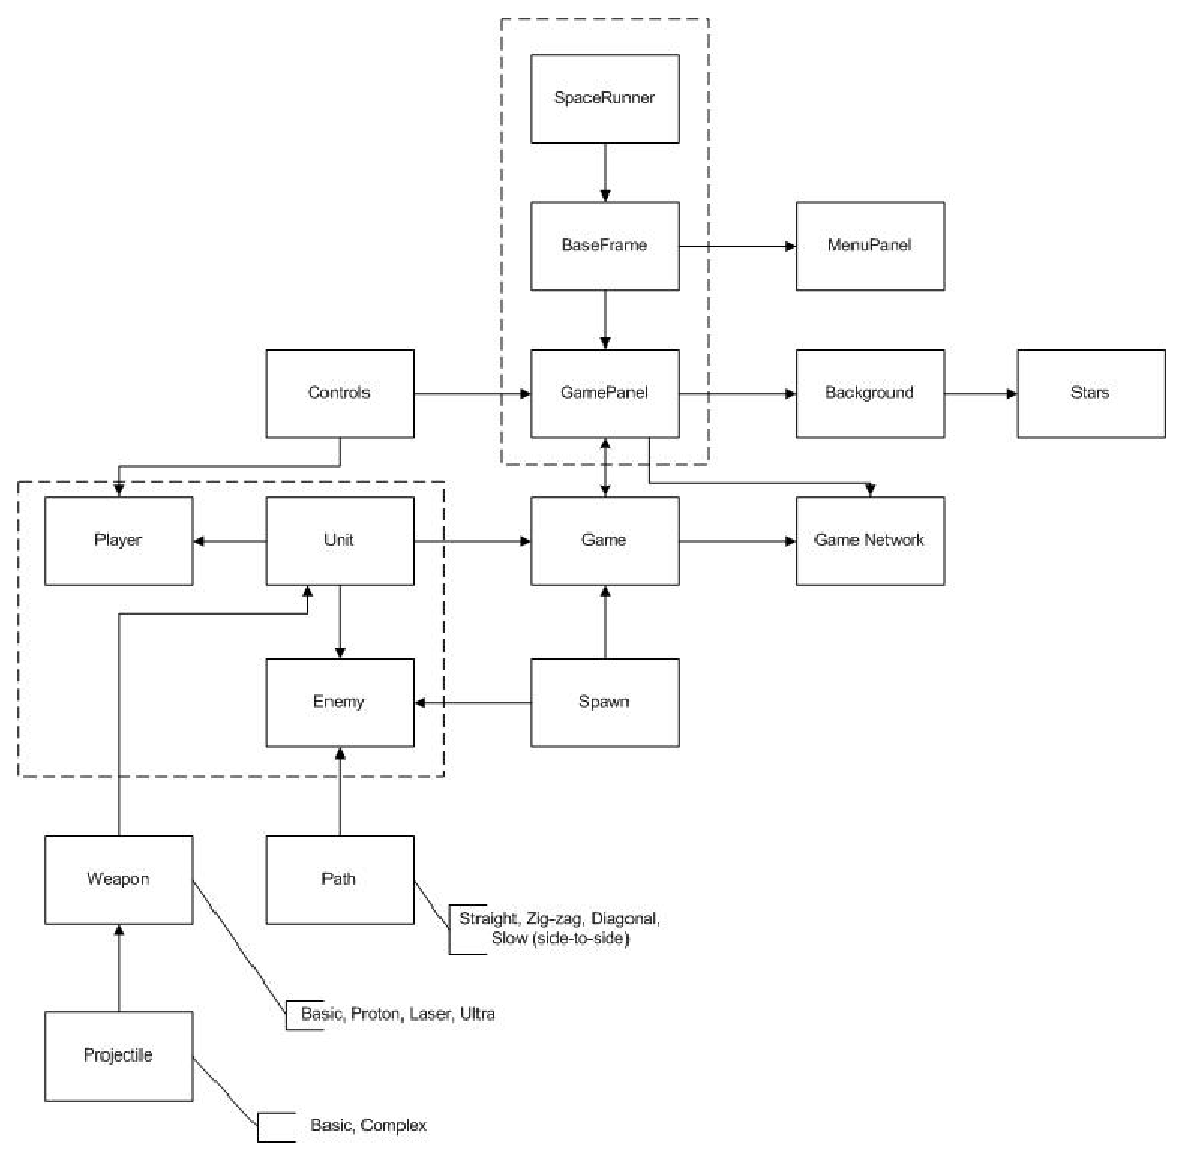
\includegraphics{class_diagram.eps}
 \caption{Proposed class diagram for the project}
 \label{fig: class_diagram}
\end{figure}

\section{Implementation}
\subsection{GUI}
\subsection{Game Logic}
\subsection{Game Objects}
\subsection{Network}


 % Dan to finish

\chapter{Validation and Testing}
\label{cha:validation}

Your applet is expected to be in good working order and do something
useful. This chapter is important, because it describes how you
assure yourself that that is the case.

\emph{Testing} is so you can be confident that the software is
robust and bug-free. What was your strategy for that? How did you
plan unit testing (for components) and integration testing (for the
whole applet)? How did the prototype fit in?

\emph{Validation} is to check that in the end the applet is useful
and pleasant to use. What was your strategy for that? Have you tried
it out with teachers or students? What kind of rolling validation
did you use for the evolutionary part (developing the GUI)?

Establish what your project can handle successfully, and what its
limitations are. Use meaningful examples, not lists of trivial
cases.
 % Michal

\chapter{Project Management}
\label{cha:management}

The week-to-week management of your project is documented in your weekly
progress reports, so you do not need to repeat that information here. A number
of important points that you need to address are:
\begin{itemize}
\item What are the main components of the project (or \emph{workpackages}) that have to be completed for it to succeed?
\item What software process model (e.g. waterfall or evolutionary)
did you use for \emph{individual workpackages}?
\item How did you allocate team members to particular tasks?
\item How did you coordinate what team members were working on?
\item How did you communicate the relevant technical information in the
team?
\end{itemize}
Note that a clean design makes all of these easier, so you could
refer to your design section, i.e. chapter~\ref{cha:design}, where
appropriate. You can also discuss difficulties in the team
interactions if there were any, and how you dealt with them.

\begin{figure}
  \centering
  \includegraphics[width=.5\textwidth]{gant}
  \caption{Example timeplan of a project.}
  \label{fig:timeplan}
\end{figure}
You can, for example, include a chart detailing the time management of your
project as shown in figure~\ref{fig:timeplan}. Explain the single workpackages
in the text:
\begin{description}
\item[Workpackage 1:] Requirements specification
  \hfill (Week 1)
\item[Workpackage 2:] Something else\ldots
  \hspace*{\fill} (Week 2---3)
\item[Workpackage 3:] \ldots
\end{description}
This is only an example chart, of course; your own timeplan will
probably look differently. Note that different workpackages can be
worked on in parallel!

Figures are included in {\LaTeX} as \texttt{.eps} files. In Linux
you can use \texttt{convert} to convert any type of graphics file to
\texttt{.eps} format.
 % Jere

\chapter{Conclusions}
\label{cha:conclusions}

After completing the coding section of the project it has been possible to evaluate how well the whole experience went.


\section{Strengths}
\label{sec: strengths}
First of all the project was a success; we were able to implement a multi-player space shooter type game within the time limit specified in the module.\\\\
The game features several items that we did not originally think we would be able to implement, these features are the background music which was added towards the end of the project, graphics for the units and projectiles which were implemented with a few weeks to go and also the boss enemies which add a new level of difficulty to the game making it more interesting.\\\\
The management side of the project was also successful as the team were very good at communicating ideas between each other. To do this the team organised weekly face-to-face meetings to openly discuss the week's work as well as evaluate what had taken place that week and what still needs to be done. Although the project may have seen to be rushed towards the end, it was still delivered on time and is playable both as a single player game but also as a multi-player networked game.\\\\
During the development of the project the team faced a setback where one member of the team had to leave the UK, despite this inconvenience the team still managed to communicate effectively through email and Facebook and didn't cause too much disruption to the project as a whole. In this scenario the team decided it would be best to break the project up into larger sections so the team member could work alone without needing as much communication with the rest of the time like the start of the project had done. This was a success and the team member managed to contribute both to the coding sections of the game as well as the final report.
\section{Limitations}
\label{sec: limitations}
Some of the game's limitations have been documented in the testing and validation section.\\\\
Although the game itself functions properly and is playable there are some slight bugs as with any software project. After playing the game for a few minutes, the number of enemies and subsequently projectiles increases. The game manages to prune the arrays containing the objects when they leave the screen but soon the game starts to slow down and become slightly unresponsive. This bug was only introduced in the last week and due to time limitations, still exists.\\\\
The project did become delayed towards the end of the project, and, although it wasn't too much of an issue there are some claims of it being 'hacked together'. No one in the team originally had any experience in network and sockets programming which was required for the game, it was decided that this part would be left towards the end of the project while we would learn more during the term through lectures and other modules. The networking section of the project does work properly, however the code is quite messy and some shortcuts have been taken. If time was not a factor this section could have been smoother and implemented better.\\\\
As previously mentioned, one of the team members had to leave the UK during the development of the project. Communication became harder as it was only possible to communicate through electronic forms such as email and Facebook rather than the preferred face-to-face meetings. It also mean't that the team member was not present for the final demonstration to explain their part of the code. Despite this setback the team still managed to proceed with the project and the team member mentioned was able to contribute to all aspects of the project (coding and report) successfully.\\\\
There are also some other limitations that relate to the game play. The enemies all have the same path to move along (except for the boss enemies) which makes the game slightly predictable. There are other paths available to use but not method to call them, perhaps a random way of choosing a path should be implemented. Also, the mouse movement can be quite sensitive if the user is not used to it which makes collisions with enemies hard to avoid.
\section{Continuation}
\label{sec: continuation}
If the project were to be continued without a time limitation then the game could be improved. The networking side of the game could be more stable and tidy and as the project is already quite abstract perhaps certain features of the current existing game can be improved, for example the enemy paths.\\\\
During the project one team member had to be away from the UK which led to certain communication issues. If the project had no time limit the team may have decided to give that person a break until a time where they could become more involved. However, in this case the team was able to work around this problem and being forced to overcome the communication difficulties which occurred with a relative degree of ease.\\\\
Outlined in the requirements of this document is a list of future requirements which could be implemented if the team were to continue the project. However, this list isn't too long which identifies that the scope of this project isn't very large. Currently the only things the player can do is move and shoot the enemies, or to do the same thing along side a network player. The game could be improved though to become more exciting but the core principal of the game isn't very large.\\\\
Currently when the player 'dies' the game ends and displays a 'Game Over' screen (including in network play). To play the game again the user has to relaunch the program, future versions of the game could see the possibility for an endless mode (as documented in future requirements) where the user is re-spawned after they 'die' as well as having the option of a 'Play Again' button to avoid relaunching the program.
\section{Future Projects}
\label{sec: future}
From completing this project the team has learnt a lot about the processes of software engineering and development and would make changes to the way in which the software was developed in the future.\\\\
The software management aspect of the game seemed to run smoothly but actually there was more work to do than what had first been anticipated. Getting to the first version of the software (v0.1) took quite long (a few weeks), this seemed to be acceptable as it would include the core basics and would see the implementation of the base cases. It was then thought that the later sections of code would be able to be introduced without changing the code too much. One of these examples is with the networking side of the program. As mentioned previously the team had relatively little experience in sockets programming and it was decided that this section would be left until last to implement. Looking back, this was perhaps the wrong decision. The thinking behind leaving the networking until later was that the team could learn more during the term from other modules as well as programming lectures. In the future if the team had little knowledge of an important aspect of the project it would be advisable to research that field from the start and try to implement it in small steps rather than as a whole when time is running out.\\\\
The scope of the project is quite small as there is little else the user can do rather than move and shoot. Although the game is large enough for the purpose of this assignment, in future projects perhaps a different game type could be suggested. Conversely, the team all enjoyed working together to produce the game and the course has benefitted each individual for future projects. The team believes the game works well despite having some small issues but all team members are happy with the output of both the software and the report.

\bibliographystyle{plain}
\bibliography{report}

Acknowledge any code you have used (if any), and also any that was
generated automatically, e.g. by wizards.

Give correct and complete bibliographic information for any sources
cited. See the local referencing guide. For instance cite which
books on software engineering you have used, for
instance~\cite{software-design}. Use the \texttt{report.bib} file to
manage your citations.

When you \emph{quote} material from other sources, you must be
absolutely clear \emph{at the point where you quote it} exactly
which of your material is quoted and what the source is. As
explained in \cite{SoCS:plagiarism},

``Direct quotation is not particularly common in scientific writing,
as it is generally not the words that matter, but the meaning.
Normally it is preferable to rewrite someone else's ideas in your
own words, often changing the terminology and other superficial
details to suit the new context.

However, in circumstances where it is appropriate to make direct use
of the words of another person, those words should normally be
included within quotation marks and a reference to the source of the
words given in the usual way.''

\end{document}
